%!TEX root = ../thesis.tex
%*******************************************************************************
%****************************** Third Chapter **********************************
%*******************************************************************************
\chapter{Approach}
\graphicspath{{Chapter3/Figs/Raster/}{Chapter3/Figs/}}

\section{Scope}

The aim of this project focuses on improving assessments and curriculum personalisation, and does not require 
coverage of all elements in the Learning Technology Systems Architecture (LTSA, Chapter 2.2.1). 
See Figure \ref{fig:ltsa-covered} for which parts of LTSA this project will attempt to cover, and 
Table \ref{table:ltsa-bcu} for the mappings from LTSA elements to the blockchain design objects in this project.

Components such as delivery and the storage of learning resources will be out of the scope of this project. 
A blockchain is also not the ideal storage service for multimedia data such as learning content and delivery activities 
due to the inherent high latency in consensus. Security and redundancy of these data is also unnecessary. 

\begin{figure}[!ht] 
    \centering    
    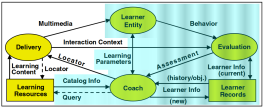
\includegraphics[width=0.85\textwidth]{ltsa-covered}
    \caption[Design Coverage of LTSA]
        {The Learning Technology Systems Architecture \citep{ieee2003ltsa}, 
        with components covered by this project highlighted in cyan} 
    \label{fig:ltsa-covered}
\end{figure}

\begin{table}[!h] 
    \caption{Mappings between LTSA elements and the BlockChain objects in this project}
    \centering
    \label{table:ltsa-bcu}
    \begin{tabularx}{\textwidth}{l|X}
        \textbf{LTSA Elements} & \textbf{BlockChain Objects}
        \\\toprule
        Learner Entity (component) & Learner
        \\\midrule
        Coach (component) & Teacher
        \\\midrule
        Evaluation (component) & Assessment Results, Feedback
        \\\midrule
        Behavior (flow) & Submission
        \\\midrule
        Catalog Info (flow) & Course Modules, Module Units
        \\\midrule
        Assessment (flow) & Assessment (Automatic Assessment, Assessor Assessment, etc.)
        \\\midrule
        Learner Info (flow) & Curriculum (a collection of Course Modules)
        \\\midrule
        Learning Parameters (flow) & Negotiation
        \\\midrule
        Learner Records (component) & Certificates, Submission, Assessment Results
        \\\bottomrule
    \end{tabularx}
\end{table}

\section{Lean Project Management and Agile Software Development}

\subsection{Project Timeline}

\begin{figure}[!hb]
    \centering
    \includegraphics[width=1.0\textwidth]{simple_gantt}
    \caption[Project Timeline]
        {A timeline of the stages of actions in this project and their dependencies if any}
    \label{fig:simple_gantt}
\end{figure}

The project largely follows a linear process, with key steps in planning, requirements elicitation, 
implementation and evaluation shown in Figure \ref{fig:simple_gantt}.
% Fairly waterfall... research specific?

\subsection{Lean Project Management}

Two kanbans were used to manage the project processes: a Kanban for implementation and 
a Kanban for research and writing. The implementation Kanban used
a loose adaptation of the development phase Kanban from \citet[p.25]{middleton2012lean}, 
without ideation, user acceptance testing and release stages.
See Table \ref{table:kanban-implementation} and \ref{table:kanban-research} for what the Kanban categories adopted are:
\\
\begin{table}[!ht] 
    \caption{Implementation Kanban used for the project}
    \centering
    \label{table:kanban-implementation}
    \begin{tabular}{|c|c|c|c|}
        \hline
        Minimum Marketable Function & Developing & Development Complete & Tested \\
        &&&\\
        &&&\\
        \hline
    \end{tabular}
\end{table}
\begin{table}[!ht] 
    \caption{Research Kanban used for the project}
    \centering
    \label{table:kanban-research}
    \begin{tabular}{|c|c|c|c|}
        \hline
        Reading/Activity & Writing & Review & Completed\\
        &&&\\
        &&&\\        
        \hline
    \end{tabular}
\end{table}

The Kanbans are drawn on the online collaborative Kanban platform Trello. This is due to 
the good extensibility of Trello, with plugins allowing the attachment of links and documents 
from many other platforms.

% \begin{figure}[!hb] 
%     \centering
%     \includegraphics[width=1.0\textwidth]{}
%     \caption[Extreme Programming]
%         {A timeline of the stages of actions in this project and their dependencies if any, loosely based on a Gantt chart} 
%     \label{fig:}
% \end{figure}

\subsection{Agile Software Development}

There are two main agile software development principles that this project has chosen to adopt:

\begin{itemize}
    \setlength\itemsep{0em}        
    \item Working software over comprehensive documentation;
    \item Responding to change over following a plan.\\
    \citep{beck2001agile}    
\end{itemize}

Some clear limitations exist, for example, \citet{beck2001agile}'s Agile Manifesto asks for 
daily collaboration between customer and developers, but contact with stakeholders 
for this project has only happen twice at the requirements elicitation 
phase and the evaluation phase. \citet{beck2001agile} also asks for teamwork and 
interactions over processes and tools, but this project is an individual endeavour.

At the end of the implementation phase of this project, two main iterations were completed.
